\section{LSM9DS1}\label{sec_design_LSM9DS1}
\textit{kursiv tekst...}
\subsection{Design}
Der benyttes et integrated circuit (IC) af typen LSM9DS1, som både indeholder magnometer, gyroskop og accelerometer, hvoraf magnometret ikke benyttes. Det er muligt at indstille accelerometeret til $\pm$1, $\pm$4, $\pm$8 eller $\pm$16 g, og gyroskopet kan indstilles til $\pm$245, $\pm$500 eller $\pm$2000 grader per sekund. \citep{Jimb02016} \newline
LSM9DS1 har ni frihedsgrader, hvilket betyder, at den måler i x-, y- og z-aksen for både magnometret, gyroskopet og accelerometeret, som kan ses på \figref{vores_IC}. %Akserne for gyroskopet og accelerometeret internt følger højrehåndsreglen.
\citep{Jimb02016}\newline 
\begin{figure}[H]
	\centering
	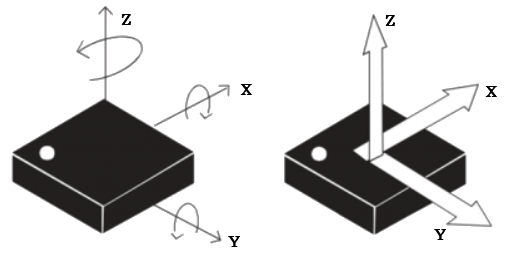
\includegraphics[scale=0.6]{figures/cDesign/LSM9DS1.png}
	\caption{På figuren ses akserne fra LSM9DS1. Til venstre ses magnometret, hvis akser er drejet én omgang i forhold til de to andre sensorer. I midten ses gyroskopet med sine roterende akser og til højre ses accelerometerets akser.\citep{Jimb02016}}
	\label{vores_IC}
\end{figure}
LSM9DS1 er en digital sensor, hvormed de analoge signaler konverteres til digitale i IC'en. De digitaliserede signal kan både bruges med en SPI og en I$^{2}$C styrefunktion, hvor mikrokontrolleren CY8CKIT-043 PSoC 4-M besidder begge. Der ønskes at benytte I$^{2}$C funktionen, da IC'en både skal sende og modtage data.\fxnote{Modtage om gyroskopet skal tændes eller slukkes.} For at benytte I$^{2}$C funktionen sættes pin CS\_AG høj, og de fire pins SDO og CS benyttes ikke. Alle pins kan ses på \figref{IC_pins}. Før et signal kan registreres kobles pinnen GND til jord, og på benet VDD skal der leveres mellem 1,9 V og 3,6 V.\fxnote{skriv resten af opsætningen efter at have snakket med John}. 
\begin{figure}[H]
	\centering
	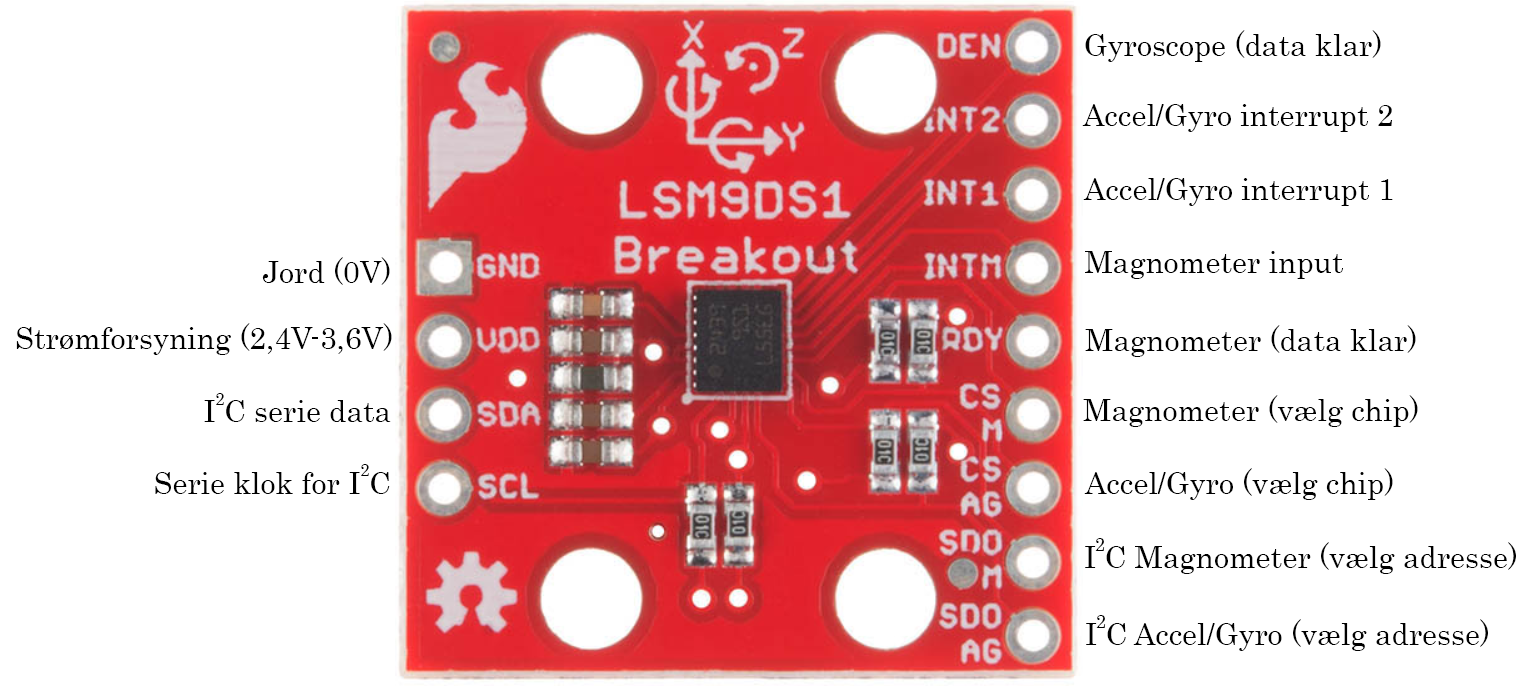
\includegraphics[scale=0.35]{figures/cDesign/accelerometeret.png}
	\caption{På figuren ses udgangene fra IC'en.\citep{Jimb02016}}
	\label{IC_pins}
\end{figure}
I LSM9DS1 bruger gyroskopet 4 mA og accelerometeret bruger 600$\mu$ A ved normale betingelser, hvor Vdd er forsynet med 2,2V og temperaturen er 25 grader. Det er derfor væsentligt, at gyroskopet bruges minimalt, når systemet skal være batteridrevet. Det er muligt enten at slukke begge sensorer, at benytte accelerometeret alene eller benytte både accelerometeret og gyroskopet sammen, hvor de har samme mængde output af data. Der kan yderligere spares strøm ved brug af gyroskopet, hvis der vælges en lavere samplerate. % alt efter hvor hurtigt et signal skal samples. 
Gyroskopet har tre forskellige power modes: slukket, low power og normal power. For at gyroskopet kan være i low power, skal outputtet af data være på 14,9-119 Hz. Hvis outputsignalet er over dette, vil gyroskopet automatisk gå i normal power. 

Accelerometeret og gyroskopet har 32 åbninger af 16 bit data FIFO til hver af gyroskopets akser, samt 16 bit FIFO til hver af accelerometerets akser. Derved skal data ikke konstant sendes til en enhed og der kan spares strøm. Bufferen kan virke på fem forskellige måder, hvor der er tre overordnede tilstande: Bypass tilstand, FIFO tilstand og kontinuert tilstand, som alle tre er illustreret på \figref{tilstand}. Derudover er der to kombinerede tilstande: kontinuert-til-FIFO tilstand og bypass-til-kontinuert tilstand. \newline

\begin{figure}[H]
	\centering
	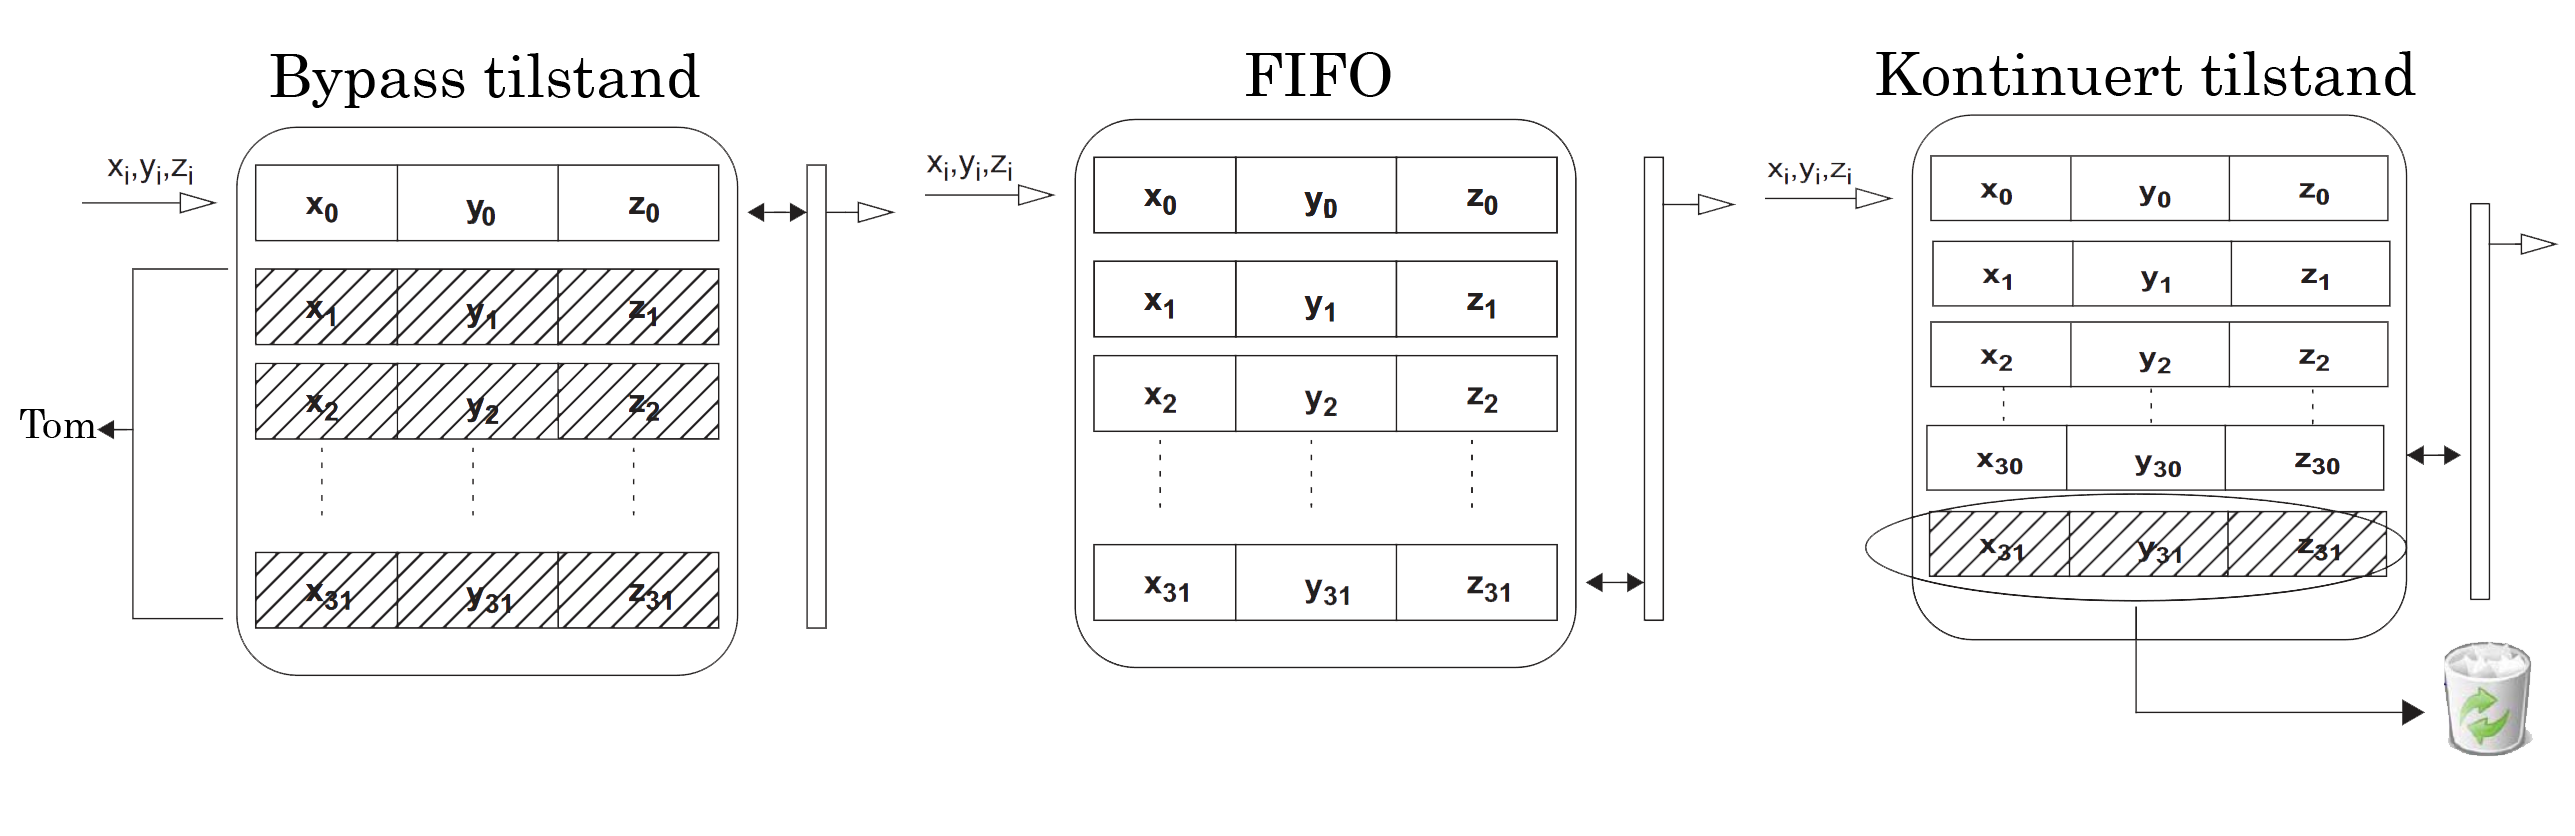
\includegraphics[scale=0.28]{figures/cDesign/LSM9DS1_tilstand.png}
	\caption{På figuren ses de tre overordnede tilstande IC'en kan opsamle data med.\citep{Jimb02016}}
	\label{tilstand}
\end{figure}

I bypass tilstanden bruges kun den første adresse, som overskrives når ny data er tilgængelig. Denne tilstand benyttes blandt andet til at nulstille FIFO
FIFO stilstanden bruges til at lagre data i niveauer indtil ny data overskriver det gamle. Det er muligt at gemme data i 32 niveauer, men dette kan tilpasses mindre efter behov. For at gammel data ikke overskrides indsættes et interrupt når FIFO er fyldt, hvormed der ikke lagres ny data. 
Den kontinuerte tilstand muliggør kontinuert FIFO, hvormed ny data overskriver gammel data. 
Ved kontinuert-til-FIFO tilstand skifter tilstanden alt efter de bit der modtages i interruptet for accelerometeret og gyroskopet. Hvis der modtages et bit på 1 vil den være i FIFO tilstand, og modtages der et bit på 0, vil den være i kontinuert tilstand. 
I bypass-til-kontinuert tilstand skiftes der ligeledes mellem bypass og kontinuert tilstand alt efter det modtagne interrups for accelerometeret og gyroskopet. Hvis der modtages et bit på 1, er den i kontinuert tilstand, og modtages der en bit på 0, nulstilles den ved at gå i bypass tilstand. 
